\chapter{Results And Discussion} \label{chapter:results}

% Chapter introduction
In this chapter we apply the framework established in \mbox{Chapter \ref{chapter:exp-setup}} to the \acrshort{fspm}s we selected in Chapter \ref{chapter:models-used}.
With this framework, we tested the reservoir characteristics of each of the physiological processes in Table \ref{table:simulation_reservoirs}.
We first study the linear input separation for physiologically relevant regression tasks.
Then, we examine the fading memory property of the considered physiological processes. 
Finally, we point out some weaknesses in our methods and how they could have been mitigated.


\section{Input Separation} \label{results:input-sep}

% Introduction input separation
We used several regression tasks to test the linear input separation in the physiological reservoirs.
These tasks fall into three categories: (i) predicting current environmental conditions, (ii) predicting the plant's eco-physiological performance, and (iii) computational benchmarks.
For the reservoir readout, we used a random sample of the plant structure, with a size of 32 and 7 for HydroShoot and CN-Wheat, respectively.
We considered 16 different random reservoir samples for each plant model to determine the performance variability caused by the selected observations.


\subsection{Environmental Inputs and Physiological Tasks}

% Input and physiological task regression scores
Let us first consider categories (i) and (ii).
For the environmental targets, we considered air temperature ($T_{\text{air}}$), relative humidity (RH) and incident photosynthetically active radiation (PAR).
We chose these targets because of their physiological relevance and to compare the results with those already obtained for strawberry plants in \citet{pieters_reservoir_2022}.
For the physiological targets we used transpiration rate ($E$), absorbed PAR ($\Phi_{\text{PAR}}$) and net photosynthesis rate ($A_n$). 
$A_n$ was only available in HydroShoot.
% The latter was only available in HydroShoot.

Figure \ref{fig:input-phys-scores} showcases the performance of each physiological reservoir as boxplots.
For the HydroShoot model, we observe that each reservoir performs roughly the same for a given target.
In CN-Wheat, the difference between the reservoirs is more outspoken.
For example, RH correlates relatively well with $E$ in CN-Wheat, where none of the processes in HydroShoot correlate well with RH.
We must also note that CN-Wheat significantly outperforms HydroShoot in most tasks.
% This disparity can partly be attributed to the larger relative observability of the CN-Wheat model; 
% for CN-Wheat, we observed \SI{70}{\percent} of the structural elements compared to only \SI{8.9}{\percent} for HydroShoot.
% The impact of observability is particularly noticeable in $\Phi_{\text{PAR}}$, where CN-Wheat achieves near-perfect accuracy with the $A_n$ and $E$ reservoirs.

\begin{figure}[hp]
	\centering
    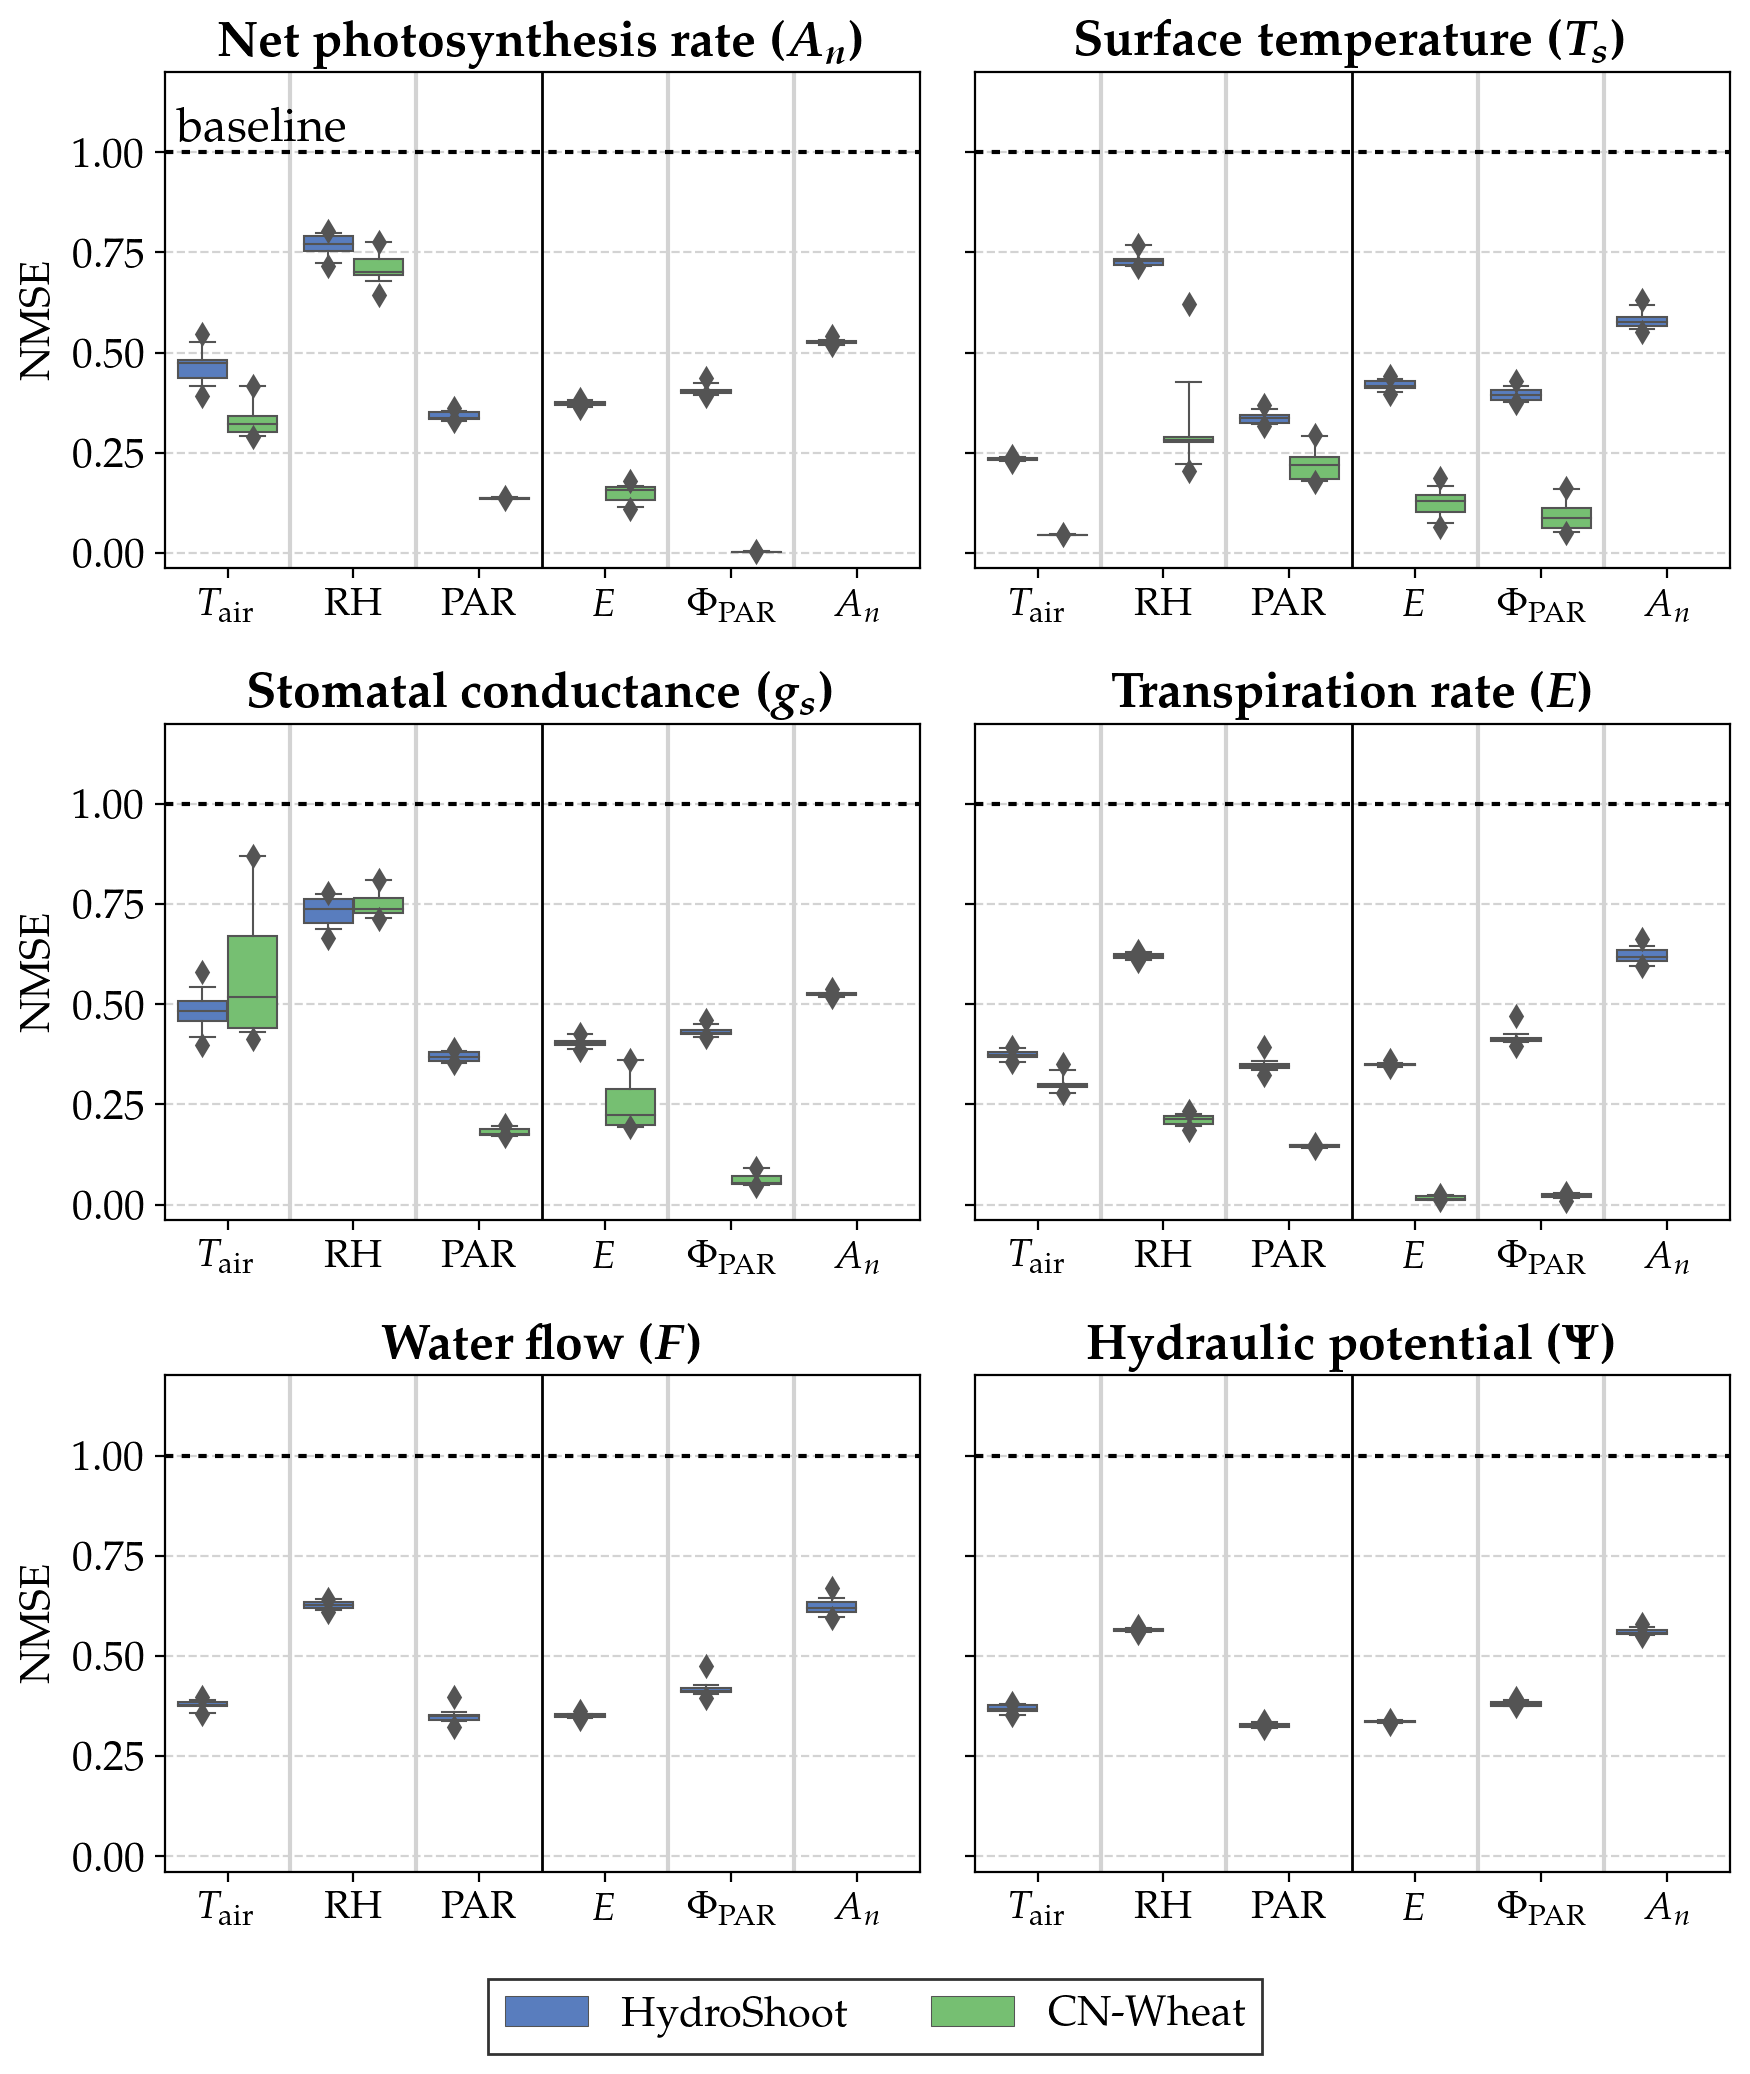
\includegraphics[width=0.82\textwidth]{img/regression_res_perf.png}
	\caption[Reservoir performance for input and physiological regression tasks.]
	        {Reservoir performance for input and physiological regression tasks.
	         The different plots show the prediction accuracy (y axis) for a suite of regression tasks (x axis) for each of the physiological reservoirs from \mbox{Table \ref{table:simulation_reservoirs}}.
	         The regression target of net photosynthesis rate  $A_n$ was only available for the HydroShoot model.
	         Each boxplot shows the distribution of test across 16 random reservoir samplings.
	         The box shows the quartiles of the distribution; the whiskers indicate the 5th and 95th percentiles.
	         Outliers are shown as a diamond shape.}
	\label{fig:input-phys-scores}
\end{figure}

% 	- *Caption:*
% 		- To measure the variance of the regression scores caused by the choice of observed plant elements, we used 16 random reservoir samplings and calculated
% - *Discussion boxplot figure:*
% - explanation of box plot whiskers etc.


% Regression predictions input and phys.
We study the time series prediction accuracy more closely in \mbox{Figure \ref{fig:predictions-input-phys}}.
In this figure, we see that the $E$ reservoir captures the broad dynamics of PAR and $\Phi_{\text{PAR}}$ for both HydroShoot and CN-Wheat.
However, HydroShoot cannot reproduce finer details, underpredicting the highest values and overpredicting the lowest values.
Moreover, the model's predictions sometimes lag behind the target (\mbox{Figure \ref{fig:predictions-input}}, samples A and C), other times the predictions lead the target (\mbox{Figure \ref{fig:predictions-input}}, sample D).
In contrast, CN-Wheat's transpiration rate captures finer details much better.

% Regression predictions input and phys.
\begin{figure}[hp]
    \begin{subfigure}[b]{\linewidth}
    	\centering
        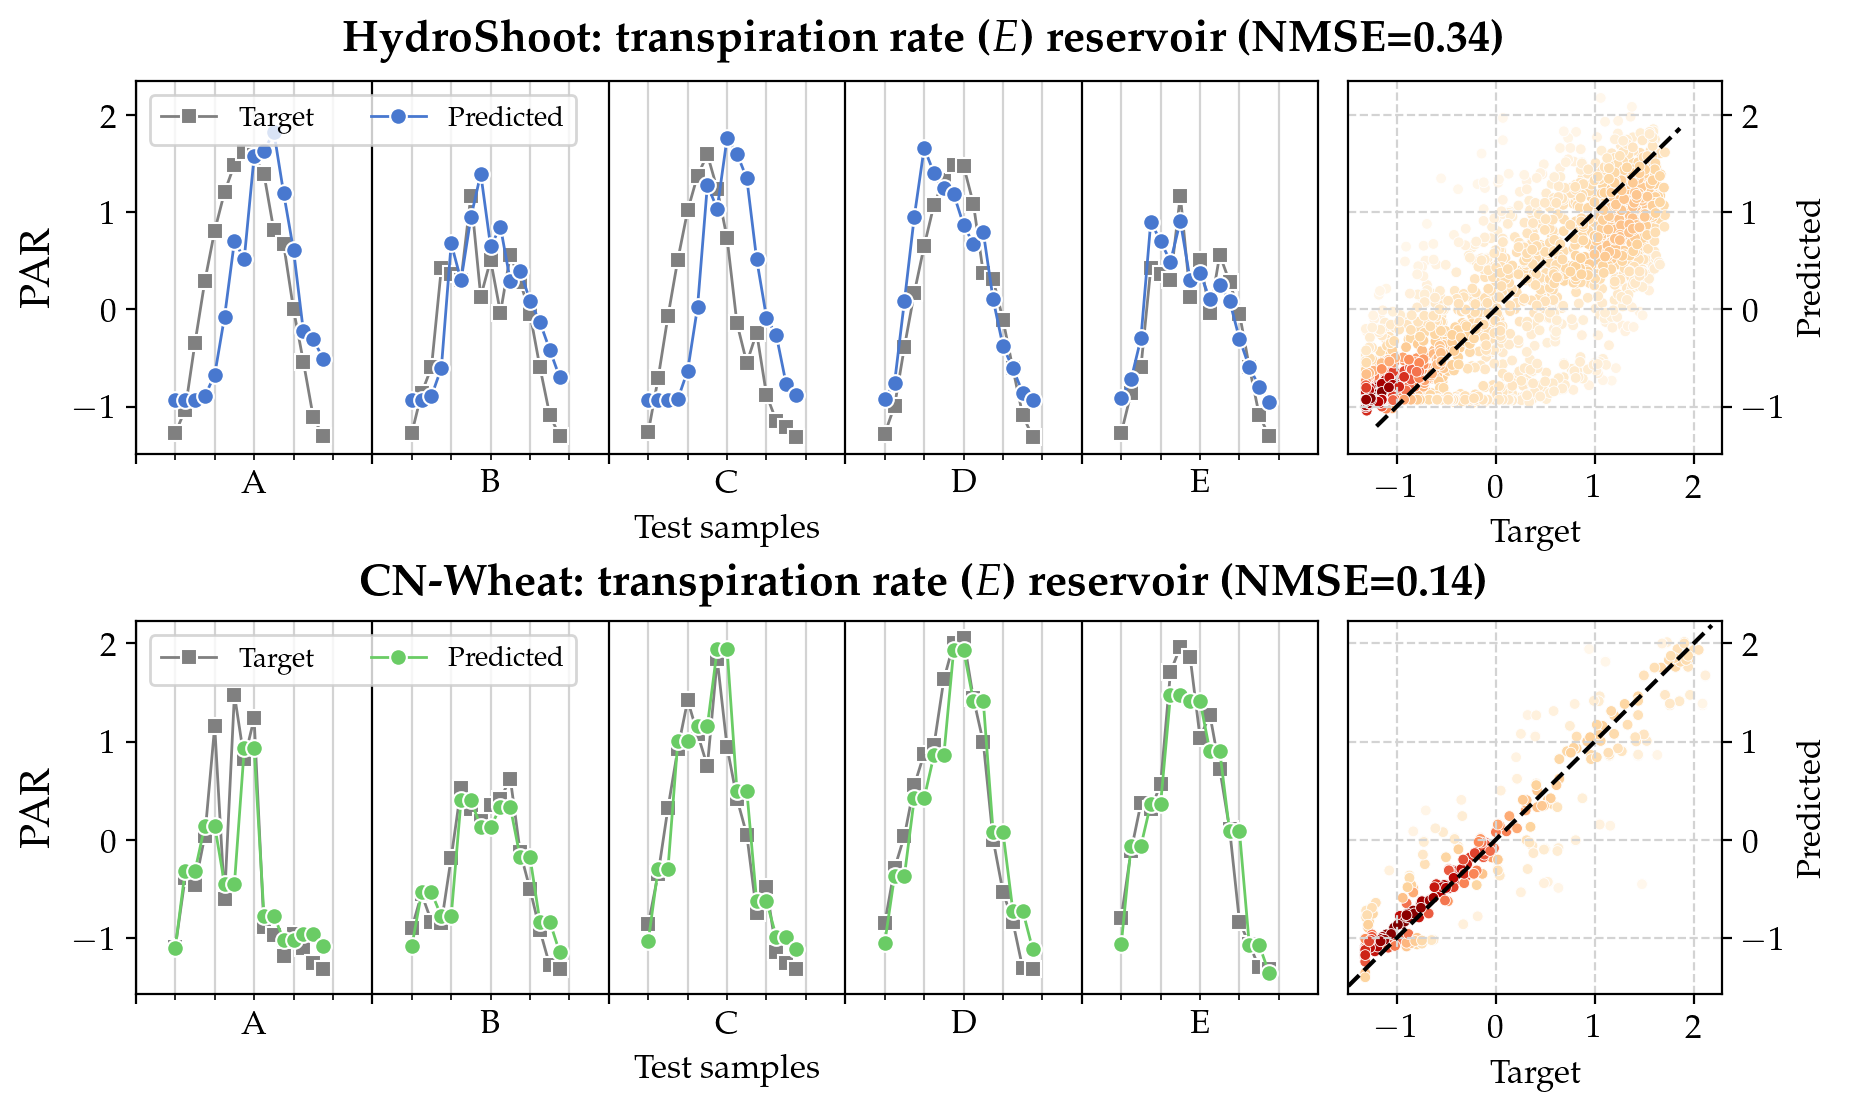
\includegraphics[width=\linewidth,keepaspectratio]{img/regression_res_prediction__input_PARi__state__Tr.png}
        \caption{Time series prediction of input PAR.}
    	\label{fig:predictions-input}
	\end{subfigure}
	\vskip\baselineskip
	\begin{subfigure}[b]{\linewidth}
	    \centering
        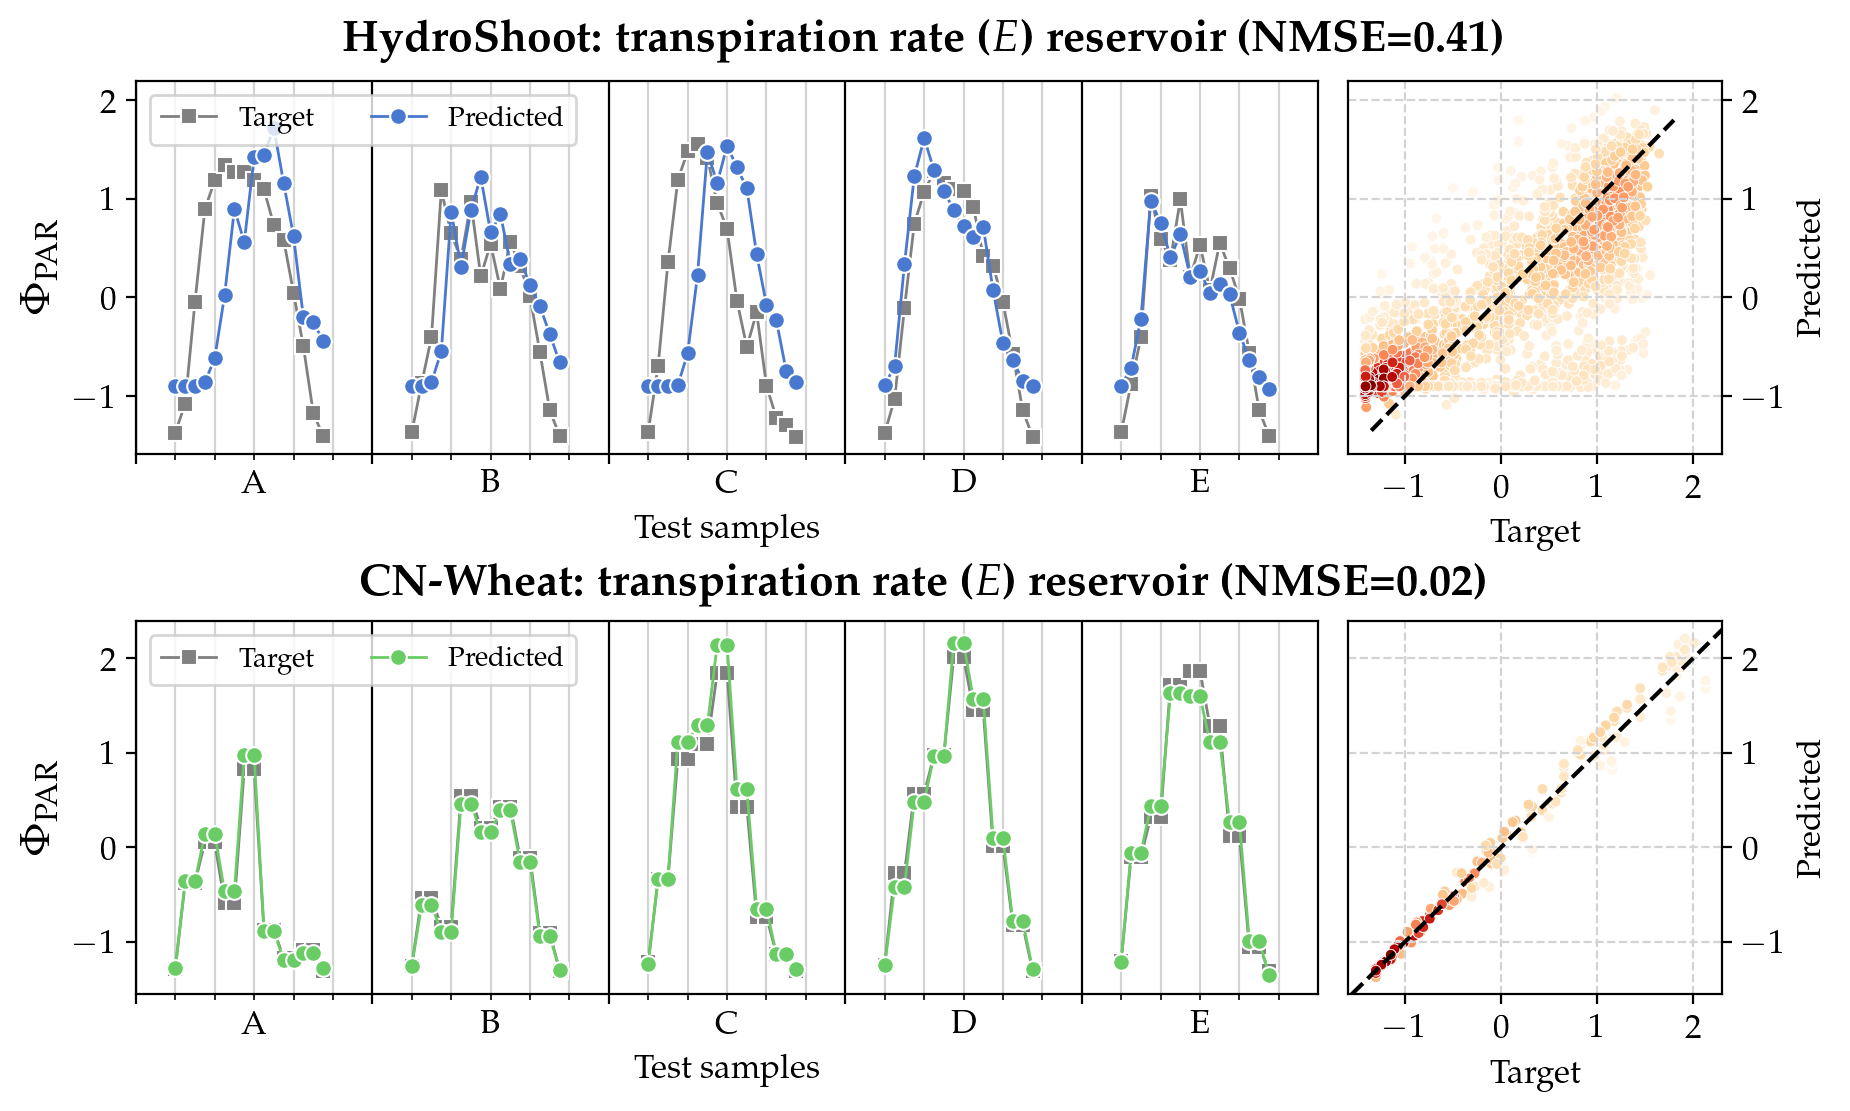
\includegraphics[width=\linewidth,keepaspectratio]{img/regression_res_prediction__output__custom__PARa__state__Tr.png}
        \caption{Time series prediction of absorbed PAR.}
    	\label{fig:predictions-phys}
	\end{subfigure}
	\caption[Time series prediction of input PAR and absorbed PAR using transpiration rate ($E$).]
	        {Time series prediction of input PAR and absorbed PAR using transpiration rate ($E$).
	         The left plot shows time series prediction for five random samples from the test set (see \mbox{Section \ref{sec:train-test-split}}),
	         the right shows the correlation between the target and predicted values. Darker colors indicate a greater density of points.}
	\label{fig:predictions-input-phys}
\end{figure}

% 	- *Caption:*
% 		- Left plots: time series prediction for five random samples from the test set (see Section 6.4).
% 		- Right plots: Correlation between target values and predicted values.
% 			- Points above the dashed line are overpredictions, points under it are underpredictions.


\subsection{Computational Benchmarks}

% Introduction
Next, we discuss the results for the computational benchmarks.
We present results for the delay line, polynomial expansion and \acrshort{narma} benchmarks based on two different input signals ($T_\text{air}$ and PAR).
For each benchmark, we compared the reservoir's advantage (or disadvantage) over a linear model of the input signal as we increased the benchmark's difficulty.
% we identified surface temperature ($T_s$) and transpiration rate ($E$) as the best performing reservoirs for these artificial tasks. 
In what follows, we discuss the results for the surface temperature ($T_s$) and transpiration rate ($E$) reservoirs specifically.


% Delay line performance of selected reservoirs
Figure \ref{fig:delay-line-scores} shows the results for the delay line benchmark.
Both reservoirs display memory capacity for solving this particular task.
For the $T_\text{air}$ input, one explanation for the observed memory is thermal inertia.
During the diurnal cycle, heat transfers between the air and the plant's water mass, which has a higher heat capacity than air.
This difference in heat capacity results in a slowed reaction to changes in ambient temperature.
The readout function can exploit this inertia to learn about past inputs.
Note that this is only a first-order interpretation, as it, for example, does not account for heat lost in evaporation.
A similar hypothesis can explain the results for incident PAR, as solar radiation affects the plant's temperature.
Lastly, we note that the transpiration rate shows similar performance characteristics as the surface temperature, indicating a possible relationship between the two processes.

\begin{figure}[t]
	\centering
    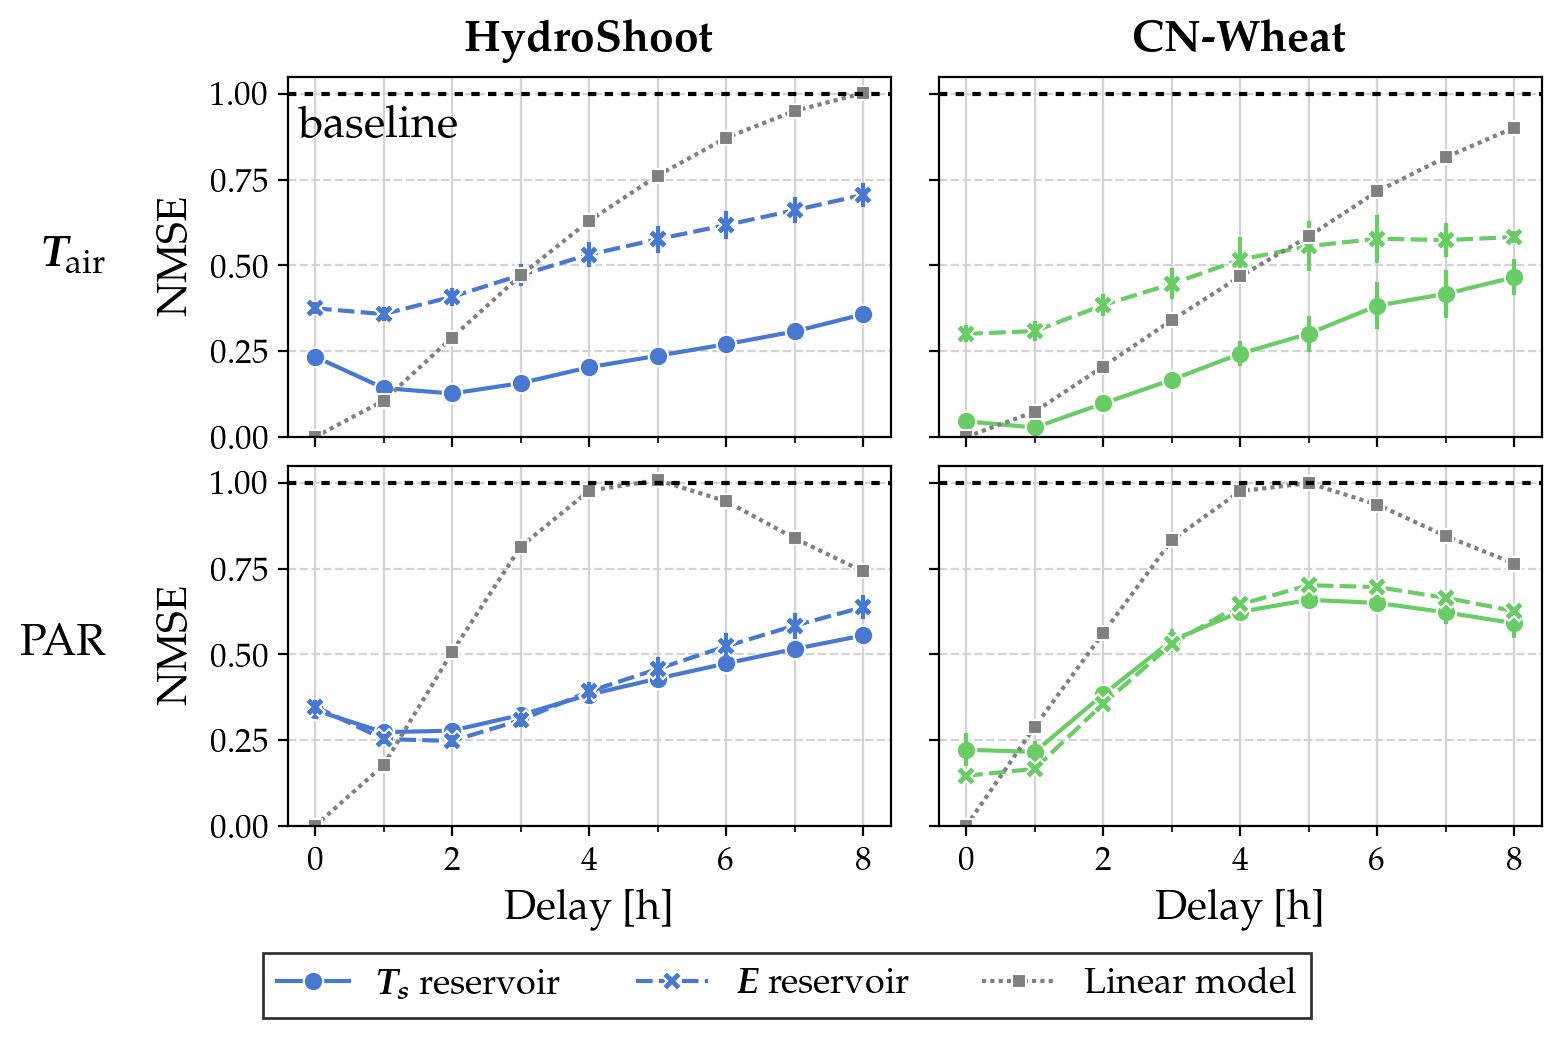
\includegraphics[width=0.82\textwidth]{img/comp_delay_perf.png}
	\caption[Predicting a time-delayed signal of $T_{\text{air}}$ and PAR using surface temperature ($T_s$) and transpiration rate ($E$).]%
    {Predicting a time-delayed signal of $T_{\text{air}}$ and PAR using surface temperature ($T_s$) and transpiration rate ($E$).
    In each plot, we compare the reservoirs' performance with a linear model that uses the benchmark's input as the only feature.
    The error bars show the scores' standard deviation.}

	\label{fig:delay-line-scores}
\end{figure}


% Polynomial task performance of selected reservoirs
Next, \mbox{Figure \ref{fig:poly-task-scores}} presents the accuracy predicting a polynomial expansion.
Interestingly, we observe a possibly polynomial relationship between the air temperature and the respiration rate, as the prediction error reaches a minimum for a degree of five.
For the other input-reservoir pairings, we see a similar performance characteristic as the linear model of the input signal, plus a bias penalty induced by the noisy relation between the reservoir and the input.

\begin{figure}[hp]
	\centering
    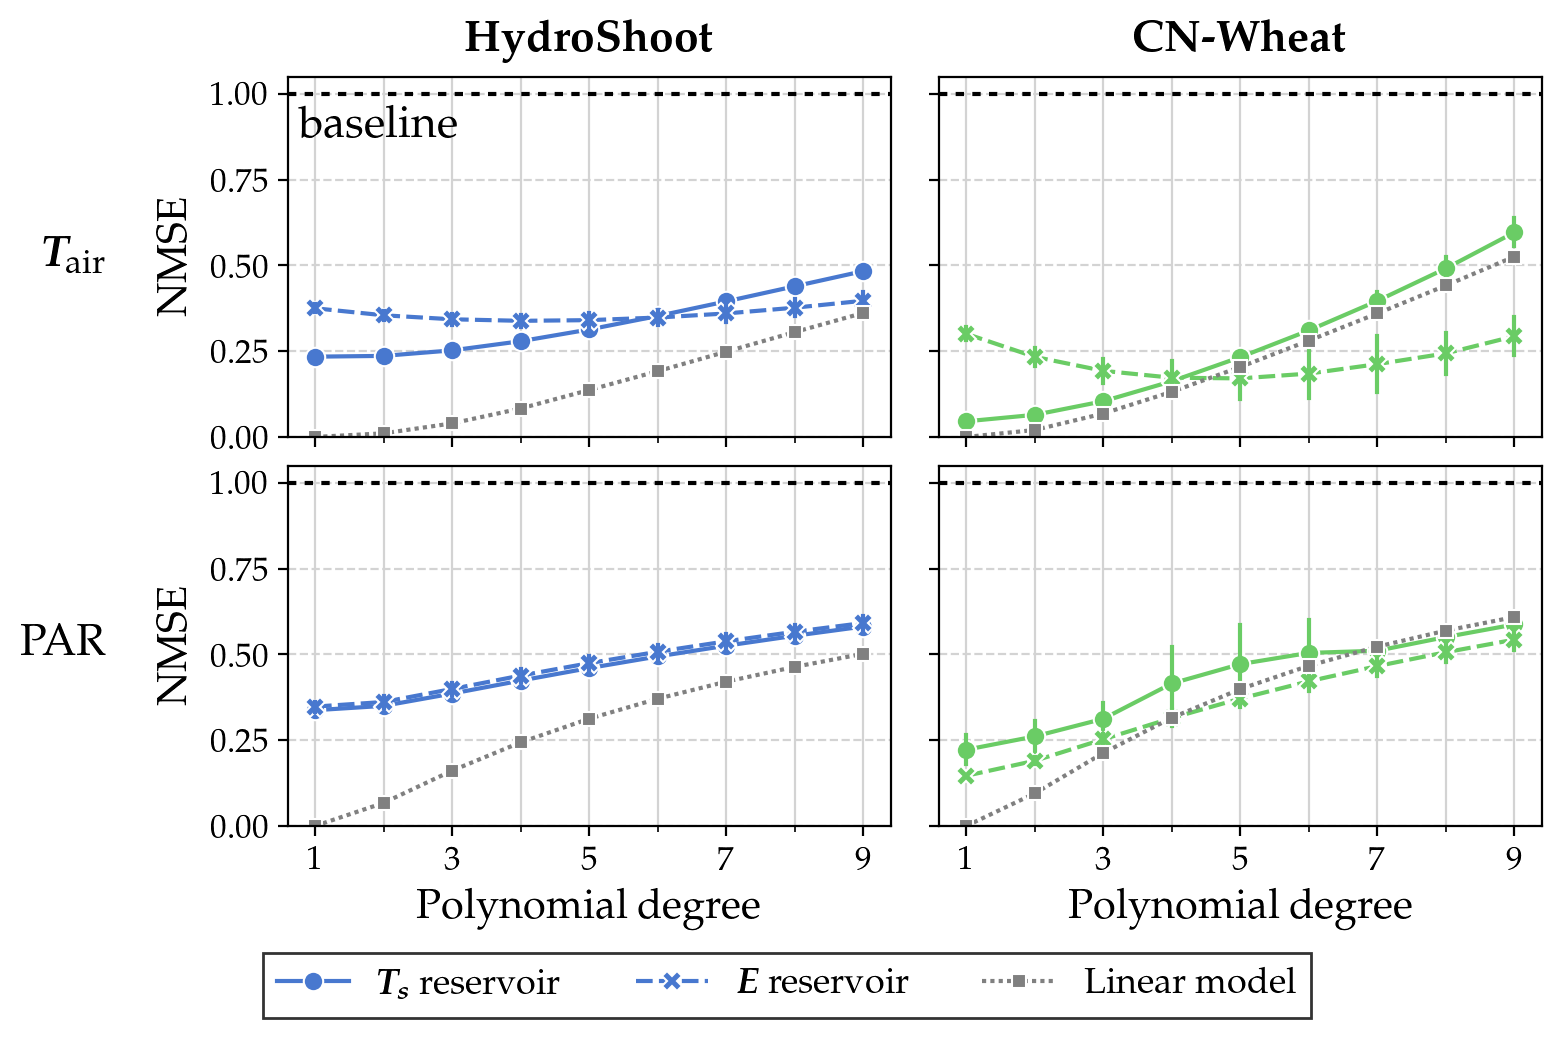
\includegraphics[width=0.82\textwidth]{img/comp_polynomial_perf.png}
	\caption%
	    [Predicting a polynomial expansion of $T_{\text{air}}$ and PAR using surface temperature ($T_s$) and transpiration rate ($E$).]%
	    {Predicting a polynomial expansion of $T_{\text{air}}$ and PAR using surface temperature ($T_s$) and transpiration rate ($E$).
	    In each plot, we compare the reservoirs' performance with a linear model that uses the benchmark's input as the only feature.
	    The error bars show the scores' standard deviation.}
	\label{fig:poly-task-scores}
\end{figure}


% NARMA benchmark performance of selected reservoirs
Finally, we consider the \acrshort{narma} benchmark.
In \mbox{Figure \ref{fig:narma-scores}} we increased the $n$ parameter from 2 up to 24. 
This means that, for $n=24$, the NARMA system integrates inputs from up to 24 hours in the past.
For the benchmark based on air temperature, only the $T_s$ reservoir outperformed the linear model. 
The same thermal inertia theory from the delay line task can explain this reservoir's correlation with this task.
Both surface temperature $T_s$ and transpiration rate $E$ outperform the linear model for the benchmark based on incident \acrshort{par}, particularly for $n$ values 8, 12, and 18.
The two reservoirs display similar performance for this task, further hinting at a relationship between the two.
From $n=18$ onwards, the performance of both the baseline model and the reservoirs improve over smaller values of $n$.
This can be explained as follows.
The input of the NARMA formula (\mbox{Equation \ref{prc:narma}}) has a period of twenty-four steps.
Setting $n=24$ means integrating over an entire day-night cycle in the formula.
This summation term then shows low variance as the input temperature and incident PAR have relatively constant cycles in our experiments (see the input data in \mbox{Appendix \ref{app:meteo}}).
The result is a smoothed, low-variance NARMA signal, which becomes easier to predict even with a linear model.
\mbox{Figure \ref{fig:predictions-narma}} shows the time series prediction for the NARMA8 task based on incident PAR, as predicted by surface temperature $T_s$.


\begin{figure}[hp]
	\centering
    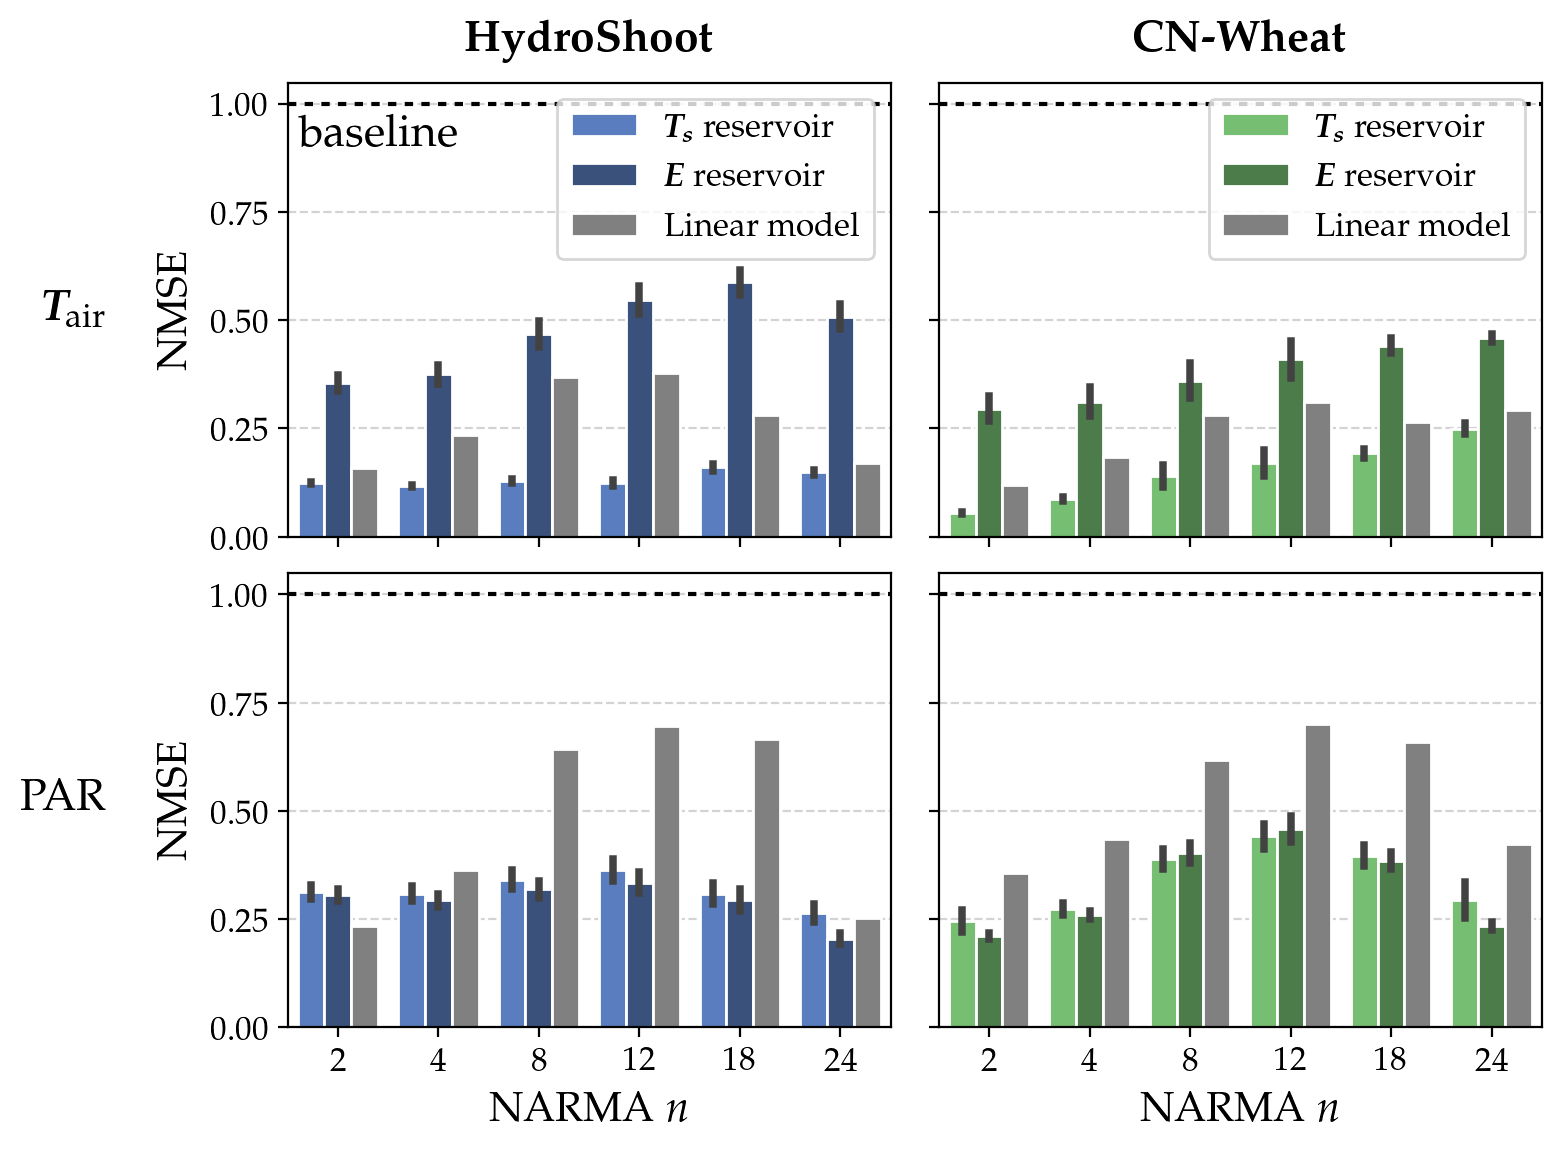
\includegraphics[width=0.82\textwidth]{img/comp_NARMA_perf.png}
	\caption[Predicting the NARMA benchmark based on $T_{\text{air}}$ and PAR using surface temperature ($T_s$) and transpiration rate ($E$).]%
	{Predicting the NARMA benchmark based on $T_{\text{air}}$ and PAR using surface temperature ($T_s$) and transpiration rate ($E$).
	In each plot, we compare the reservoirs' performance with a linear model that uses the benchmark's input as the only feature.
	The error bars show the scores' standard deviation.}
	\label{fig:narma-scores}
\end{figure}

% Regression predictions NARMA
\begin{figure}[hp]
	\centering
    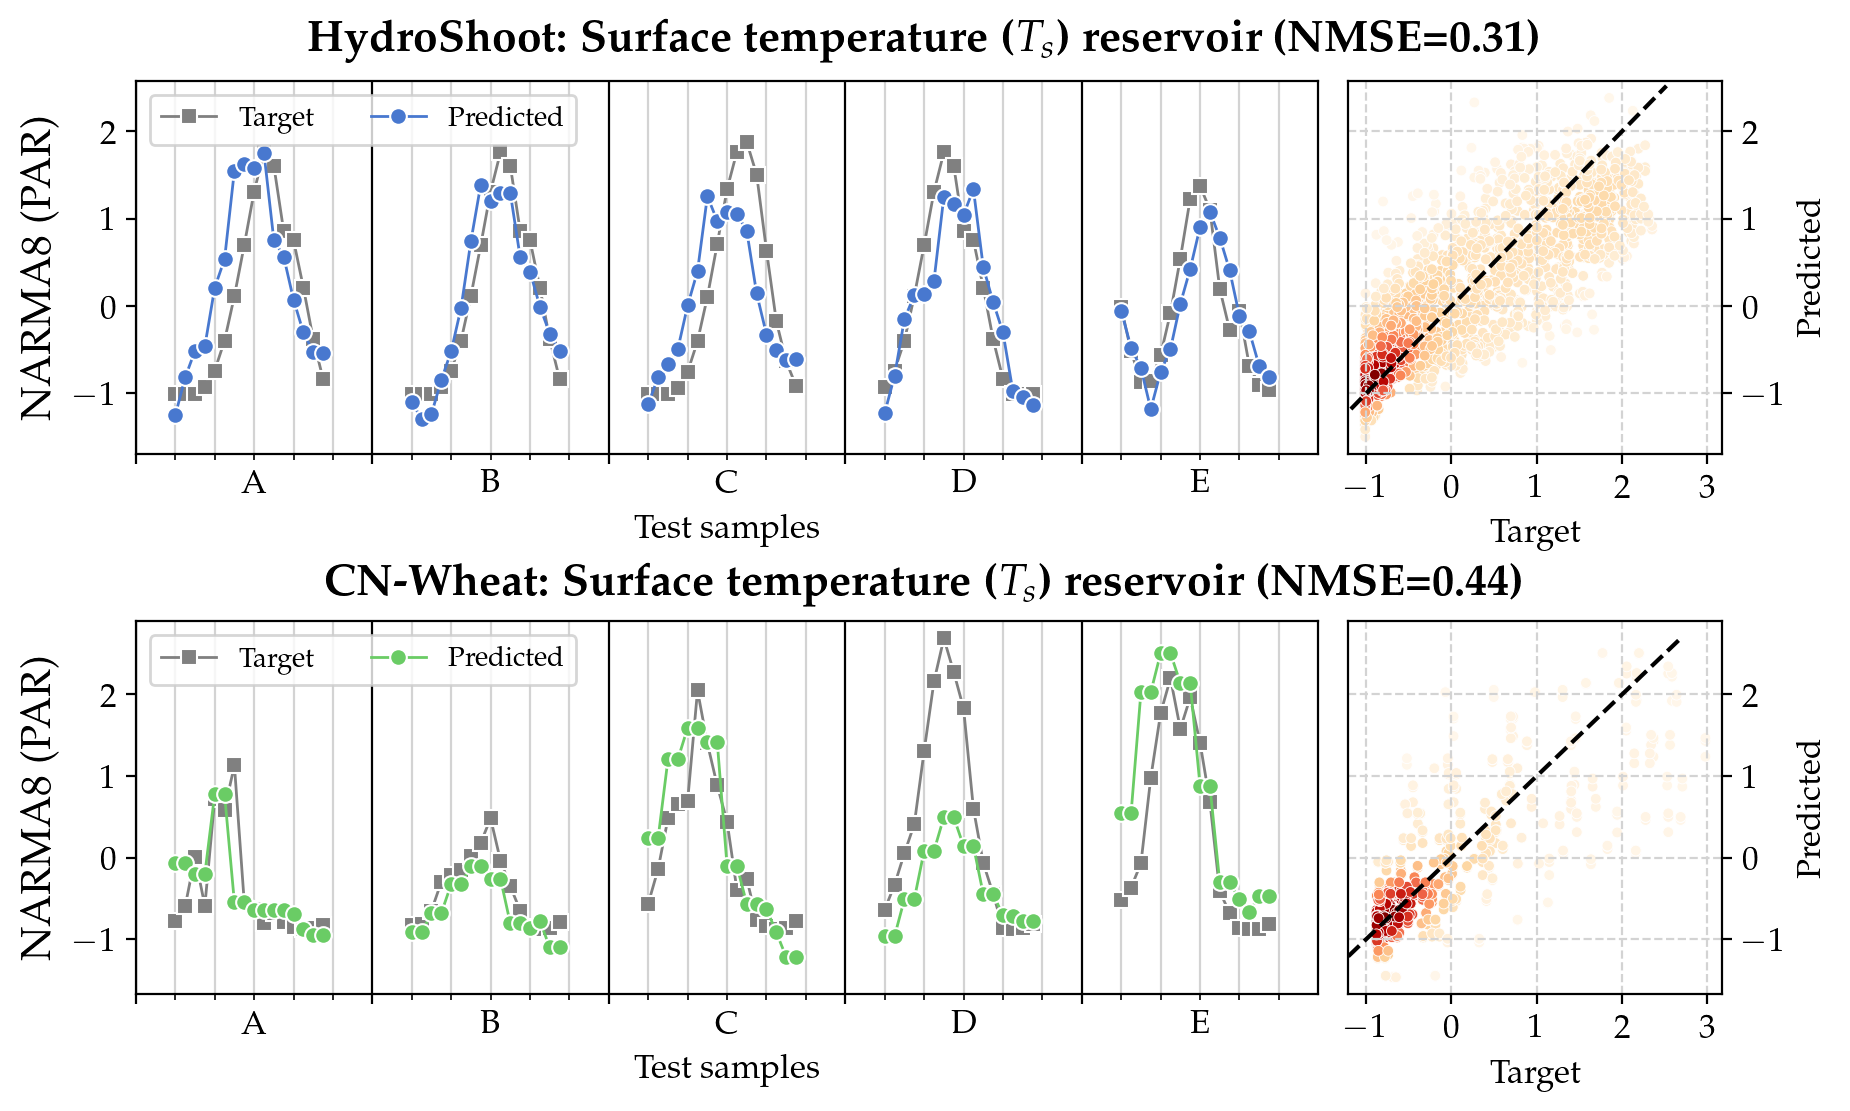
\includegraphics[width=\linewidth,keepaspectratio]{img/regression_res_prediction__input_PARi_NARMA_8__state__Ts.png}
    \caption[Time series prediction of the NARMA benchmark using surface temperature ($T_s$).]
        {Time series prediction of the NARMA benchmark using surface temperature ($T_s$).
        The left plot shows time series prediction for five random samples from the test set (see \mbox{Section \ref{sec:train-test-split}}),
         the right shows the correlation between the target and predicted values. Darker colors indicate a greater density of points.}
	\label{fig:predictions-narma}
\end{figure}

\subsection{Comparison with Previous Research}

% Comparison to Pieters 2022 results.
\citet{pieters_reservoir_2022} performed similar experiments using real-world strawberry plants.
His experiments used leaf thickness measurements of seven leaves as the observed reservoir, sampled every second.
Because leaf thickness strongly correlates with transpiration rate $E$ \citep{giuliani_coordination_2013}, we compare our results for the $E$ reservoir with the results reported using leaf thickness measurements.
We must emphasize that we are comparing prediction at different time scales; our models ran hourly, whereas Pieters' experiment was conducted at the second scale.

    The NMSE values we obtained for the input and physiological tasks are in line with what is reported by Pieters, with HydroShoot performing a bit worse and CN-Wheat a bit better than what was reported for the strawberry plant.
HydroShoot performed notably worse at predicting $E$ and $A_n$ than the strawberry plant.
However, in terms of reservoir observability, Pieters' experiment aligns closer with our reservoir for CN-Wheat than for HydroShoot.


Pieters used incident PAR as a base for the computational benchmarks, so we compare our results for that input.
We obtained significantly better results for the polynomial tasks.
The strawberry plant's prediction accuracy capped out at an NMSE of nearly 1.0 for only a degree of 6, whereas our \textit{in silico} plants achieve NMSE scores under 0.6 for up to a degree of 9.
However, our baseline linear model also performed better than Pieters' control experiment, suggesting there may be a difference in methodology that makes the tasks complicated to compare. 
The data for the delay line task can be compared for delays of 1-5 \unit{\hour}. 
Here, the results obtained in our experiments are similar to those observed for the strawberry plant.
The results for the NARMA benchmark are more difficult to compare because The NARMA task used in Pieters' work operated at the minute scale, using the alternative formulation from \mbox{Equation \ref{prc:narma-timescale-adapted}} with $\tau=60$.
Because of the hourly time step in our plant models, we designed our NARMA task at the hour scale (i.e.\ with $\tau=1$).
% The NARMA task used in Pieters' work operated at the minute scale, i.e.\ $n=100$ integrates inputs up to 100 minutes in the past.
% Because of the limited time resolution of our plant models, we designed our NARMA task at the hour scale.
We obtained significantly better results with our version of the benchmark than were reported for the minute scale task; 
The strawberry plant did not achieve NMSE values lower than 0.5 for any NARMA task.
As we explained in the previous section, this disparity may be because the NARMA task at the hour scale results in a more smoothed signal.

\section{Fading Memory}

To test the fading memory principle, we applied an impulse of varying length and amplitude to the incident \acrshort{par} of each plant model.
The experiment revealed unexpected properties in the \acrshort{fspm}s.
\mbox{Figures \ref{fig:result-impulse-cnwheat}} \mbox{and \ref{fig:result-impulse-hydroshoot}} show the divergence $\delta(t)$ (Equation \ref{methods:reservoir_divergence}) in each physiological process caused by the impulse for CN-Wheat and HydroShoot respectively.

\subsection{CN-Wheat}

Let us first study the effects of the artificial stimulus on CN-Wheat (Figure \ref{fig:result-impulse-cnwheat}).
It is immediately apparent that the reservoir's divergence changes at intervals of two hours instead of the hourly steps of the inputs.
Indeed, \citet{barillot_cn-wheat_2016-1} confirms that some submodels of CN-Wheat run at two-hour intervals to limit computational cost.
The figure indicates that the affected submodels control each of our physiological reservoirs.
On the one hand, this is unfortunate because, for our use case, the practical simulation scale is \SI{2}{\hour} instead of \SI{1}{\hour}.
On the other hand, even at this coarser simulation scale, the model was able to perform tasks well at the \SI{1}{h} scale in Section \ref{results:input-sep}. Perhaps, the results could be even more promising when simulated with an hourly time step.

Because we chose the impulse lengths to be odd, we see some misalignment between the impulse steps and the steps that show disturbance in the reservoir.
Looking past the misalignment caused by the \SI{2}{\hour} simulation interval, we see that the reservoir divergence immediately disappears when the real input signal resumes.
The most likely explanation is that the transient behavior lasts less than two hours, such that the coarse simulation steps mask any memory effects.
An alternative explanation is that the FSPM's state is a memoryless function of the immediate environmental conditions. 
We think this is unlikely because the plant model should be dynamic by construction.
We also reject the explanation that the impulse is too short to impact the reservoir because we see the same behavior resulting from a \SI{1}{\hour} or \SI{9}{\hour} stimulus.
Either way, we can safely conclude that all reservoirs in the CN-Wheat model show stationary behavior w.r.t. the PAR input as their dynamics resumed as if the impulse did not occur.

At first glance, these results for CN-Wheat seem to contradict the behavior we saw in Figure \ref{fig:delay-line-scores} for the delay line task.
We saw that $T_s$ and $E$ can predict past incident PAR better than a linear baseline model (though the scores are overall still quite bad).
An alternative explanation for this performance is that the \SI{2}{\hour} simulation steps add memory of the past hour to the reservoir for every second time step.
Figure \ref{fig:delay-line-scores} supports this theory: the reservoirs display near-identical prediction accuracy for delays of 0 h and \SI{1}{\hour} before sharply increasing for a delay of \SI{2}{\hour}.

\begin{sidewaysfigure}[hp]
	\centering
    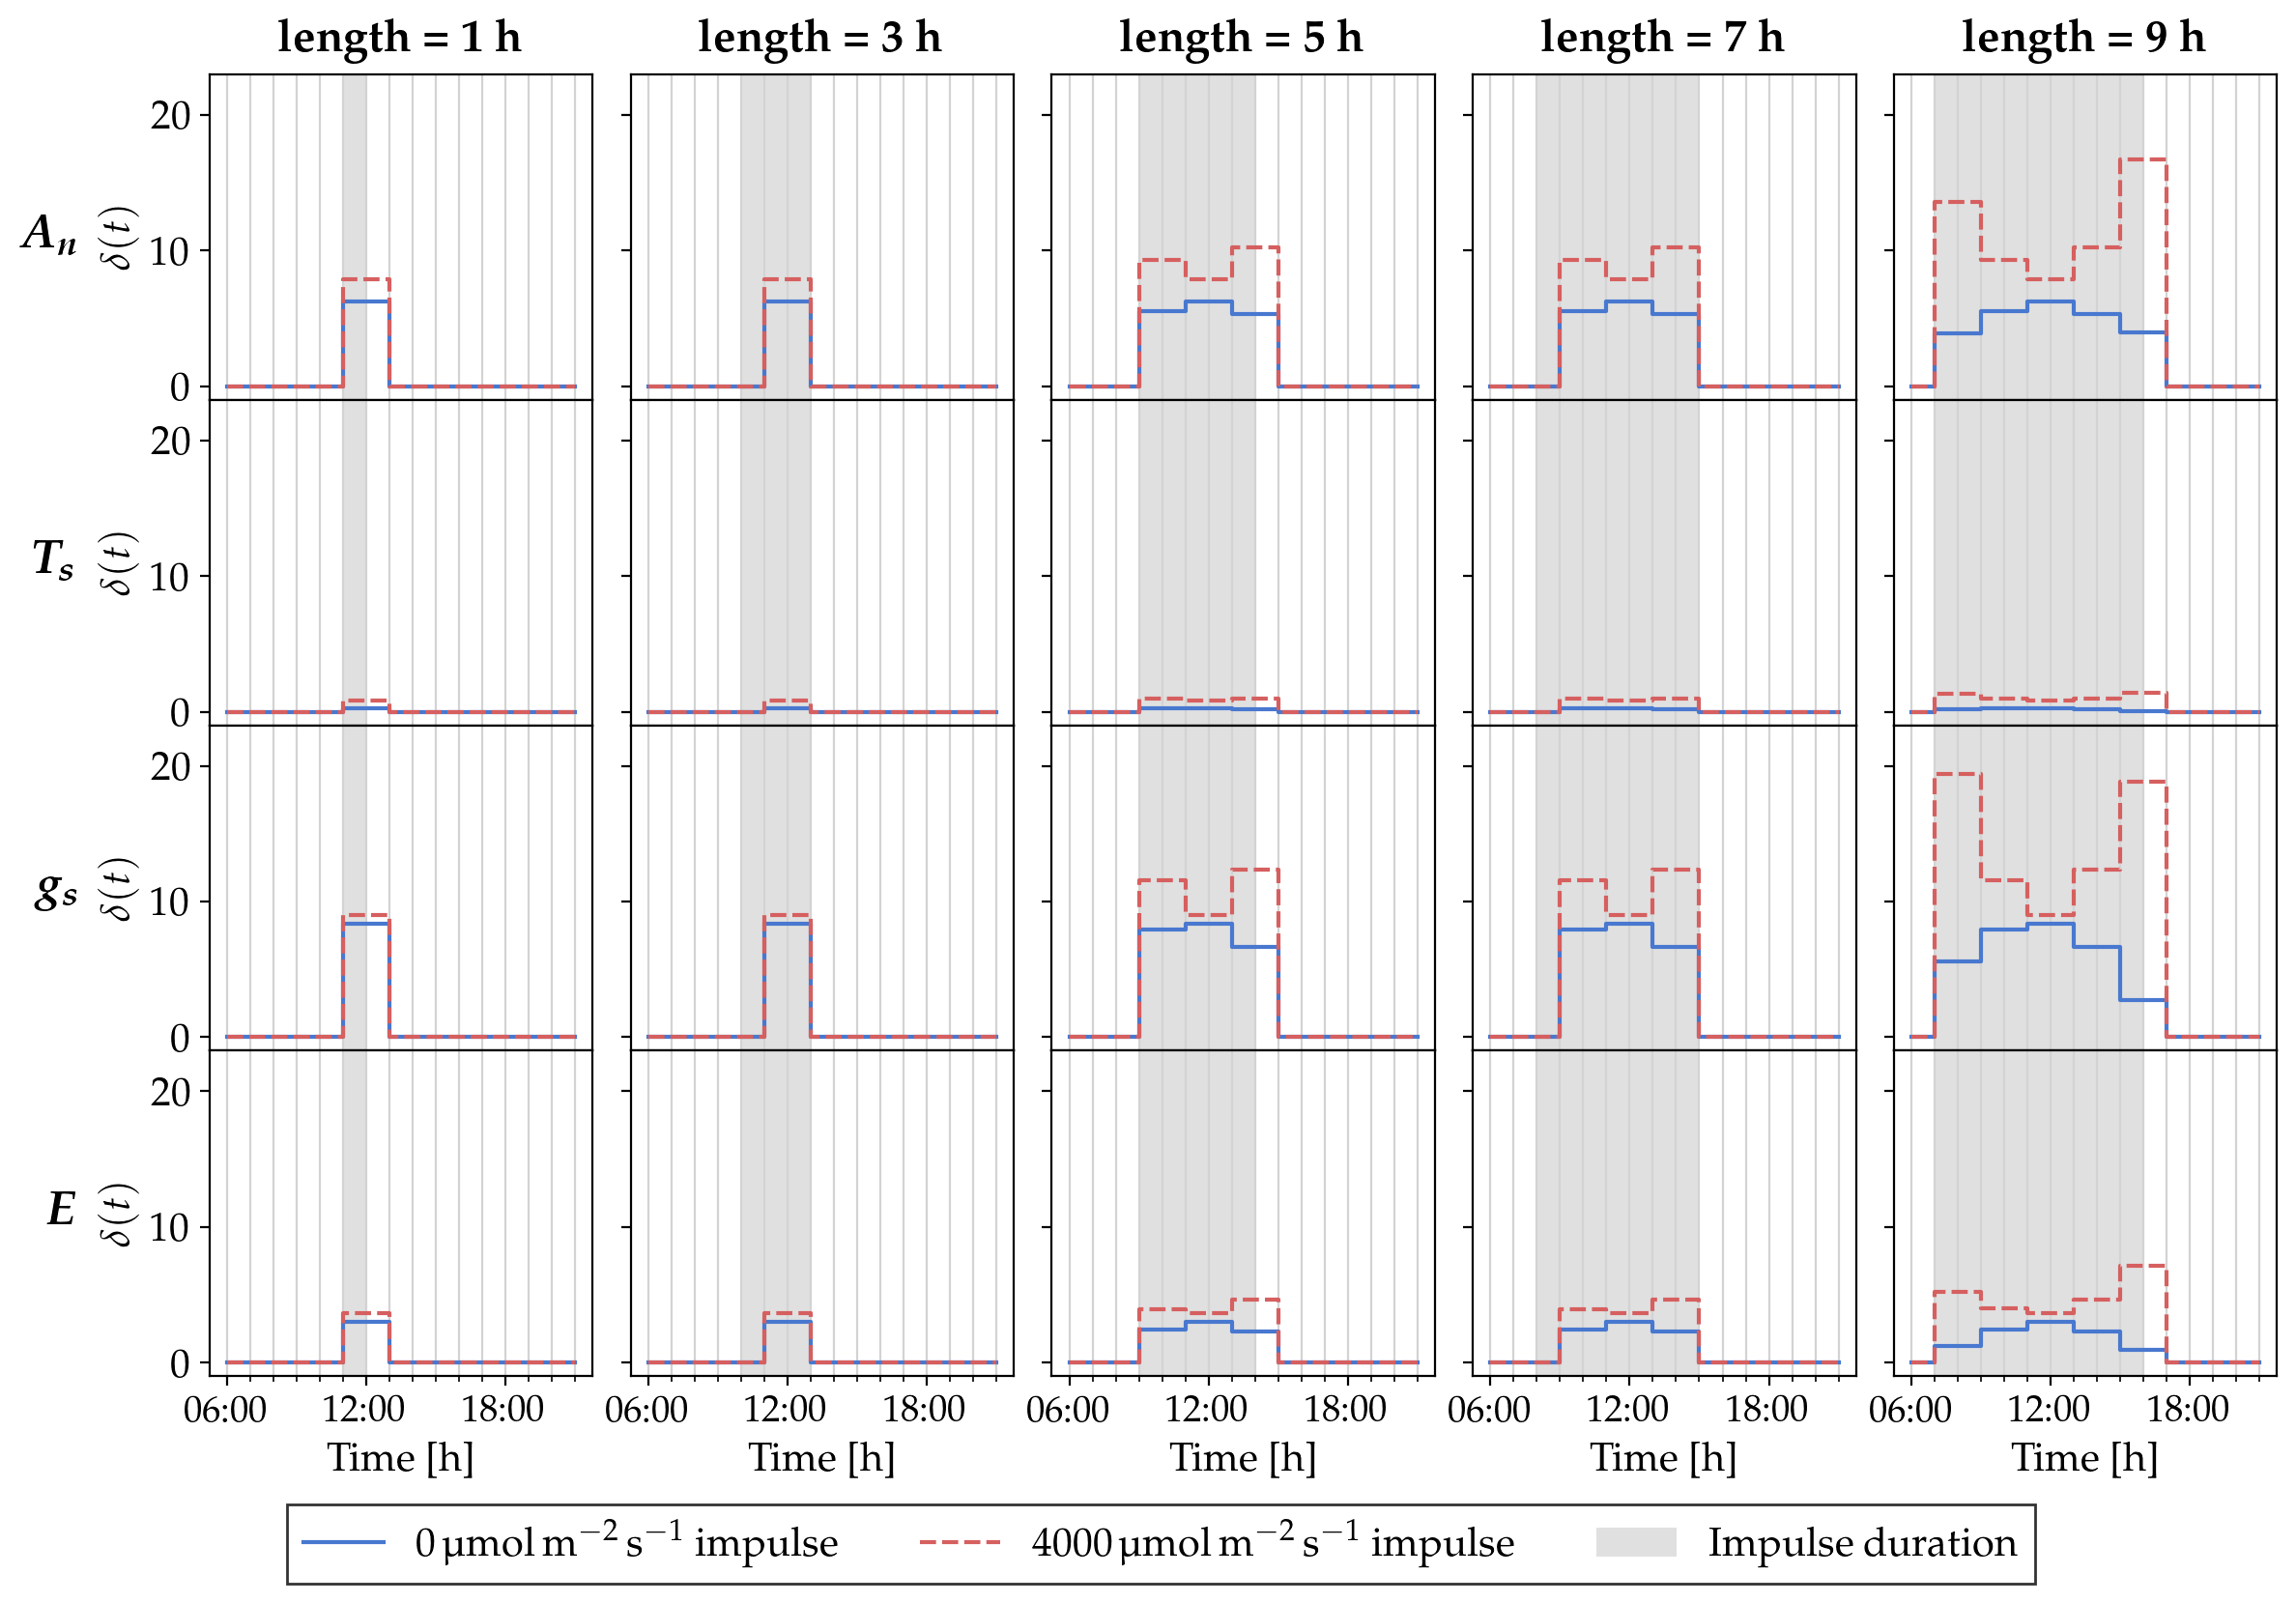
\includegraphics[width=20cm]{img/impulse_reservoirs_cnwheat.png}
	\caption{
	    CN-Wheat: Reservoir divergence $\delta(t)$ (Equation \ref{methods:reservoir_divergence}) after applying an impulse to PAR of various lengths and amplitudes.
    }
	\label{fig:result-impulse-cnwheat}
\end{sidewaysfigure}


\begin{sidewaysfigure}[hp]
	\centering
    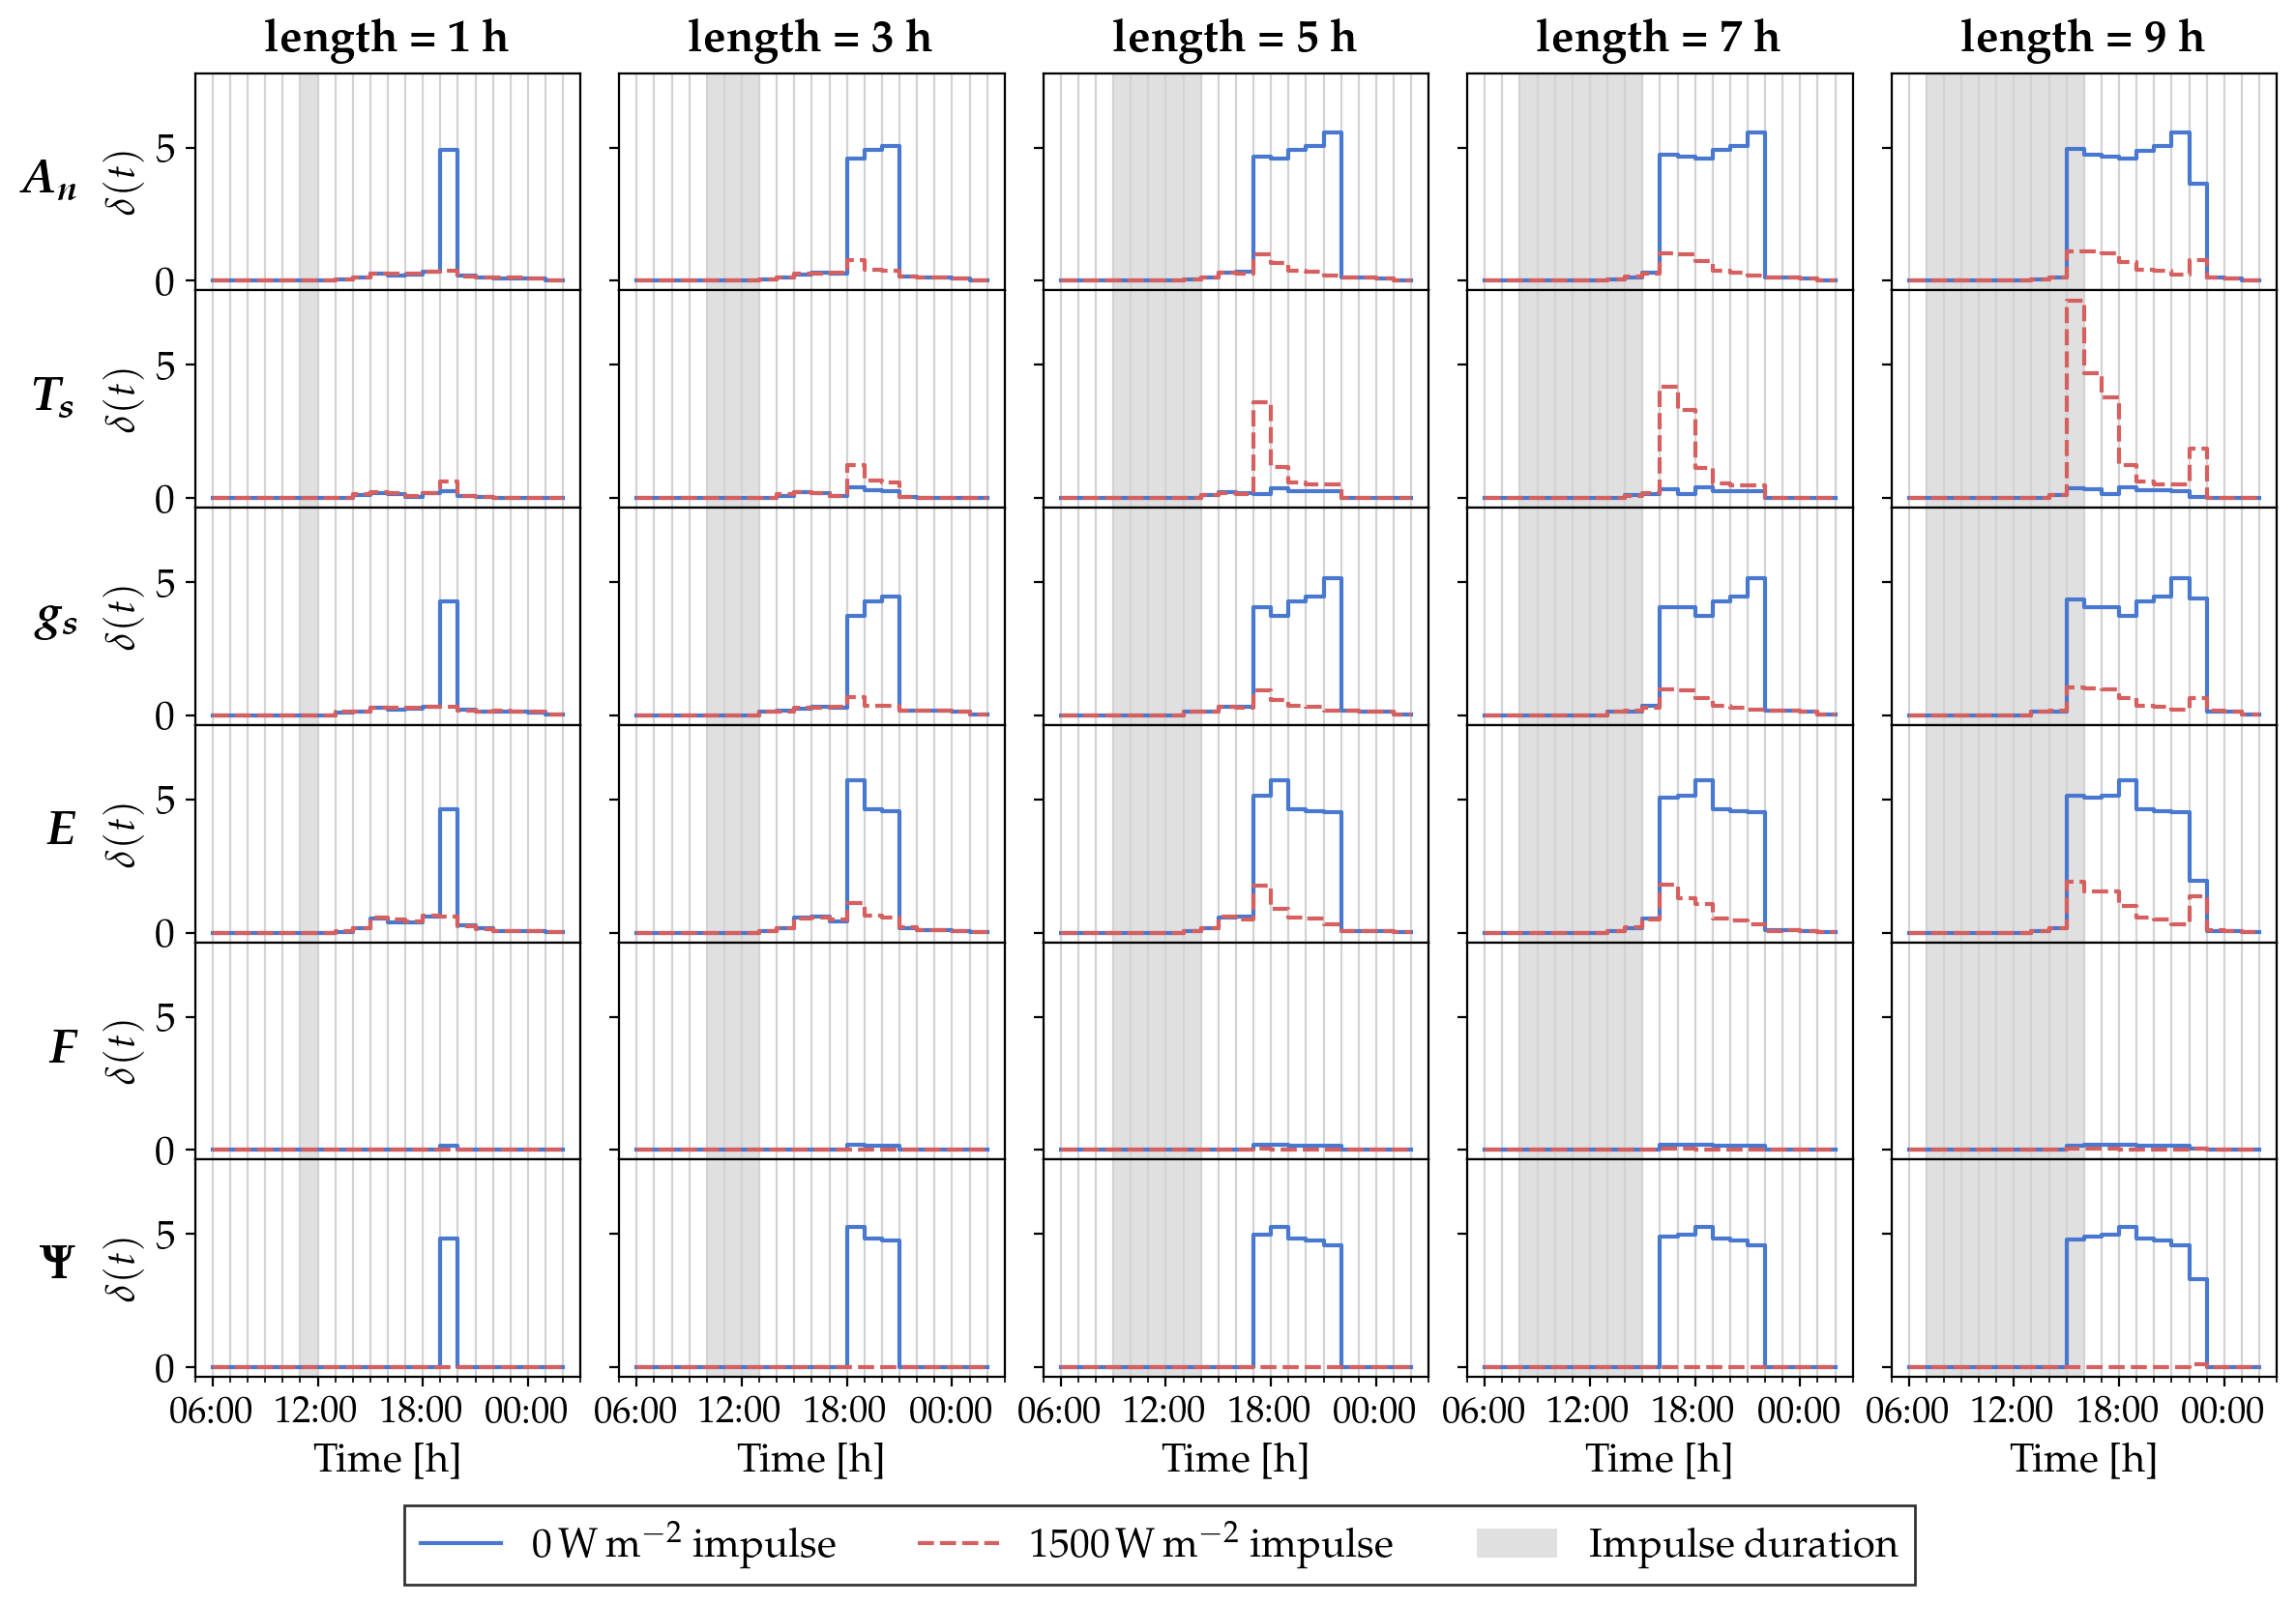
\includegraphics[width=20cm]{img/impulse_reservoirs_hydroshoot.png}
	\caption{
	    HydroShoot: Reservoir divergence $\delta(t)$ after applying an impulse to PAR of various lengths and amplitudes.
    }
	\label{fig:result-impulse-hydroshoot}
\end{sidewaysfigure}


\subsection{HydroShoot} \label{sec:results-impulse-hydroshoot}

% Hydroshoot discussion (1)
Next, we discuss the outcome of the impulse experiment for the HydroShoot \acrshort{fspm}.
Figure \ref{fig:result-impulse-hydroshoot} shows that the disturbance in the reservoir caused by the impulse in incident PAR lasts for the same length as the applied stimulus. However, the reservoir reacts at an \SI{8}{\hour} delay.
We first investigate this delayed reaction before drawing further conclusions from this data.


% Hydroshoot stability discussion (chaotic behavior)
Figure \ref{fig:hydroshoot-instability-divergence} shows the divergence metric for the entire simulation duration and compares various experimental setups.
Note that each experiment had identical initial conditions and experienced identical environmental conditions up to the start of the impulse on day 5.
The plot shows that the reservoir dynamics diverge slightly during daytime even under identical conditions.
This indicates that the observed physiological processes display somewhat chaotic dynamics during daytime hours.
Keep in mind that this cyclical divergence is quite low compared to the disturbance caused by the impulse ($\delta(t)$ of 0.4 vs. 3.5 in \mbox{Figure \ref{fig:hydroshoot-instability-divergence}}).
We did not observe cyclical divergence in CN-Wheat.
The chaotic behavior may be a result of numerical instabilities in the simulation.
However, previous reports of chaotic behavior in plant physiological processes exist in the literature.
For example, \citet{shabala_observations_1997} reported chaotic dynamics in plant physiological responses to light, which aligns with our observations.
Therefore, the chaos observed in HydroShoot may be a more realistic model than the deterministic behavior of CN-Wheat.


% Hydroshoot stability discussion (delayed responses)
Another anomaly in the HydroShoot simulation is shown in Figure \ref{fig:hydroshoot-instability-behavior}.
The figure shows a superposition of the input PAR and the mean transpiration rate of the observed reservoir elements.
The data reveals a continuously shifting misalignment between the diurnal cycle of the input signal and the oscillations in the physiological dynamics.
In an extreme example, the peak in transpiration rate lags nearly a half-period behind the incident PAR on day 4.
Comparing this data to Figure \ref{fig:hydroshoot-instability-divergence} reveals that the cyclical peaks in reservoir divergence we discussed earlier are aligned in time with these time-shifted reservoir responses.
We observed this behavior for any simulation starting day.
We were unable to identify the root cause for these dynamics, and the CN-Wheat model did not exhibit similar behavior.
This anomaly may also explain the leading and lagging predictions we observed in Figure \ref{fig:predictions-input-phys}.


% Hydroshoot discussion cont'd (2)
Continuing the analysis of the experimental results: the shifting delay in reservoir response is the most likely explanation for the delayed response to the artificial stimulus.
Since we know of the chaotic response to incident light, we must attribute the slight disturbance that precedes the delayed peak in reservoir divergence to the natural chaotic behavior and not the impulse.
Because the peak in disturbance has the same duration as the impulse and accounting for the assumed delay in reaction of \SI{8}{\hour} in the reservoir's response, we cautiously propose the same conclusion as for CN-Wheat.
That is, no lasting memory effects are visible at the simulation scale of \SI{1}{\hour}; if there are any transient dynamics, they must occur over a much shorter time frame.

% Regression predictions input and phys.
\begin{figure}[hp]
    \begin{subfigure}[b]{\linewidth}
    	\centering
        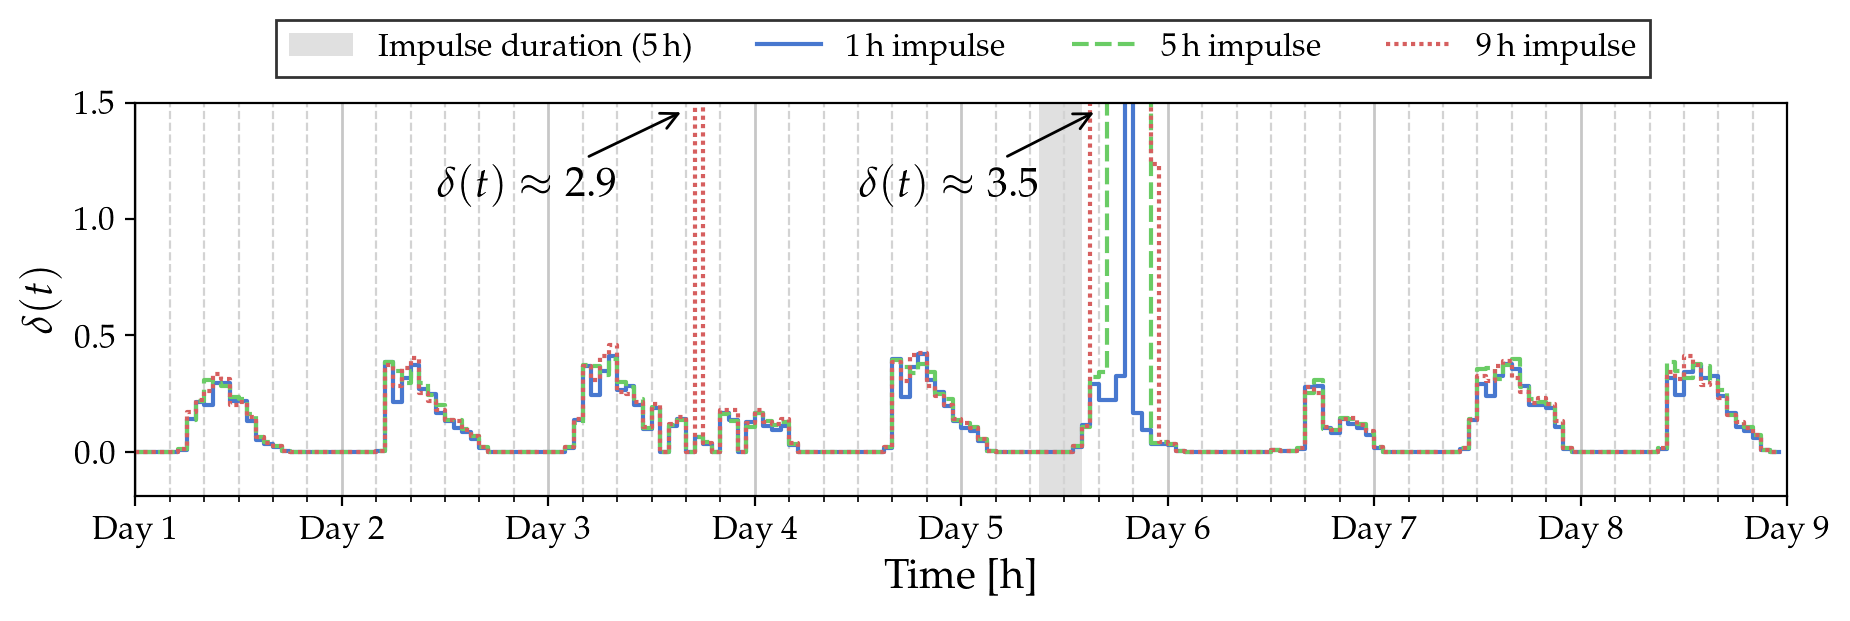
\includegraphics[width=\linewidth,keepaspectratio]{img/hydroshoot_instability_divergence.png}
        \caption{HydroShoot: Reservoir divergence $\delta(t)$ in various experiments with impulse amplitude \SI{0}{\watt\per\square\meter}.}
    	\label{fig:hydroshoot-instability-divergence}
	\end{subfigure}
	\vskip\baselineskip
	\begin{subfigure}[b]{\linewidth}
	    \centering
        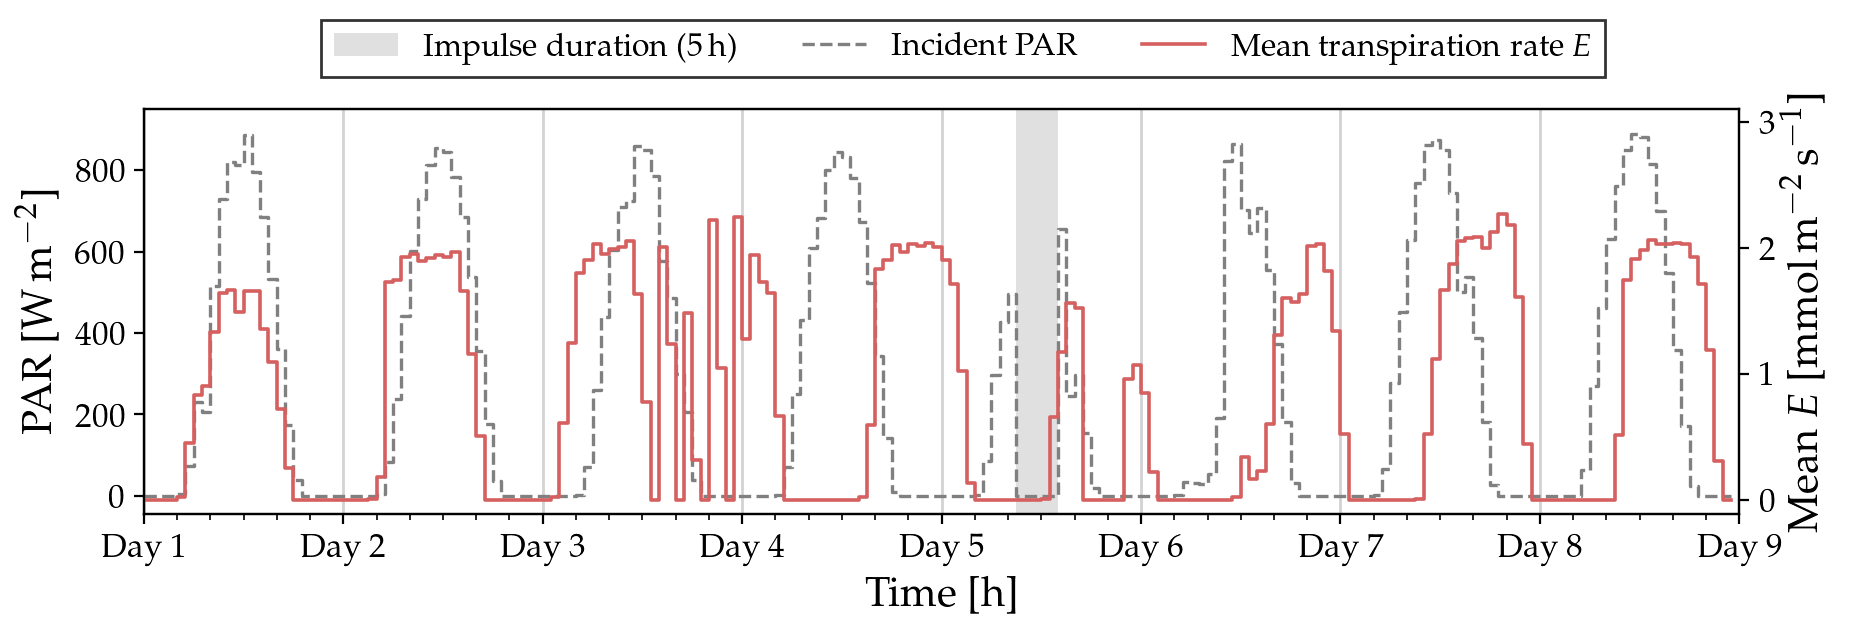
\includegraphics[width=\linewidth,keepaspectratio]{img/hydroshoot_instability_behavior.png}
        \caption{HydroShoot: Input data and modeled transpiration rate from an impulse experiment with length \SI{5}{\hour}.}
    	\label{fig:hydroshoot-instability-behavior}
	\end{subfigure}
	\caption[Two figures highlighting unstable behavior observed in the HydroShoot \acrshort{fspm}.]
        	{Two figures highlighting unstable behavior observed in the HydroShoot \acrshort{fspm}.
        	(\subref{fig:hydroshoot-instability-divergence}) 
	            Reservoir divergence $\delta(t)$ in various experiments with impulse amplitude \SI{0}{\watt\per\square\meter}.
                Under all circumstances, a cyclical pattern of reservoir divergence emerges.
        	(\subref{fig:hydroshoot-instability-behavior}) 
        	    Input data and modeled transpiration rate $E$ from an impulse experiment with length \SI{5}{\hour}.
        	    The superposition of the data reveals a shifting misalignment between the diurnal pattern of incident PAR and the consequent transpiration rate.
        	}
	\label{fig:hydroshoot-instability}
\end{figure}



% **Weaknesses:**
\section{Weaknesses in Our Methods and Potential Improvements}

% In the spirit of academic honesty, we must point out the weaknesses in our methods too.
We can identify some potential weaknesses that may have influenced our results.
For one, we used the same measurements for the reservoir as are used by the model to compute the physiological regression tasks.
This introduces positive bias into the correlation between the reservoir and the physiological targets.
This bias is especially pronounced in the accuracy of CN-Wheat for predicting total transpiration rate and absorbed PAR; 
the readout model has a distinct advantage because it could directly observe 70\% of the plant's internals.
To reduce this bias, we could have introduced some signal noise to the observations to make them less precise.
However, it is difficult to determine what amount of noise is appropriate in this case.

Another weakness is the trust we placed in the accuracy of the used FSPMs.
The authors of these plant models have only validated their accuracy for the use cases presented in their publications.
Plant models are generally not verified as one hundred percent accurate copies of their real-world counterparts.
As we observed in Section \ref{sec:results-impulse-hydroshoot}, the HydroShoot model showed some unexpected behavior that was not reported in the original paper.
To emphasize that our results characterize the behavior of plant models and not live plants, we used the names of the FSPMs throughout this chapter instead of the plant genus. 

Finally, the lack of time resolution in the plant simulations leaves us with a weak take-away about transient memory dynamics in the studied plant species.
Though we can conclude that the considered physiological reservoirs show stationary behavior at the hour scale, we cannot state the exact period for which past inputs influence the present reservoir dynamics.



\section{Summary}

In this chapter, we demonstrated the use of eco-physiological processes in computer plant models for reservoir computing.
Our results for regression tasks highlighted several promising processes that showed good predictive correlation with biologically relevant tasks.
The results can be used in future plant \acrshort{rc} research to decide which physiological processes to pursue.
The impulse experiment was less conclusive.
However, the initial results seem to imply that each considered reservoir has fading memory that lasts less than two hours, with regards to incident \acrshort{par}.
The difficulties in using the selected \acrshort{fspm}s for this experiment highlighted the need for plant models with a better time resolution than \SI{1}{h}.
Finally, through our analysis of reservoir dynamics, we observed chaotic characteristics of eco-physiological processes, as well as unexpected behavior in a plant model that was previously unreported.
Because the application of \acrshort{rc} was able to reveal these behaviors in plant models so readily, we propose that \acrshort{rc} can play a more prominent role not only in plant computation but also in the development and verification of \acrshort{fspm}s.